\scanpage{97}
map. We no longer require $\sigma_{\unsure{\widehat I|\widehat A}}$ to be without fixed points — the set of fixed points, $I$, \deleted{\unsure{itself|of}} corresponds to the ``flattened branches'' of the \inserted{$1$-}complex i.e. to the \deleted{``\unsure{ends}''} ``boundary-points'' of $X$ which are not in $S$. Giving a graph with flattened branches thus amounts (on decomposing $\widehat I$ into $I\amalg\widetilde A$, where $I=\widehat I^\sigma$ and $\widetilde A=\widehat I\setminus\unsure{\widehat I^\sigma|I}$) to giving an \deleted{\unsure{pair}} ordinary graph \inserted{$(S,\widetilde A,\sigma_{\widetilde A},o_{\widetilde A})$}, plus a set $I$ and a map $I\longrightarrow S$.

We describe such a graph with flattened branches by a drawing such as
\figure{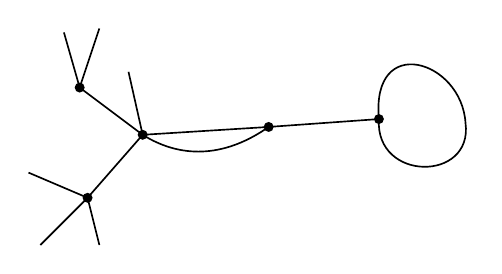
\begin{tikzpicture}[x=1cm,y=1cm,line width=.6pt]
\coordinate (a) at (0,0); \coordinate (b) at (-.8,.6); \coordinate (c) at (-.7,-.8); \coordinate (d) at (1.6,.1); \coordinate (e) at (3,.2);
\draw (a)--(b) (a)--(c) (a)--(d)--(e);
\draw (a) to[out=-32,in=-145] (d);
\draw (e) .. controls (2.9,1.3) and (4.05,.95) .. (4.1,.15) .. controls (4.2,-.6) and (2.95,-.6) .. (e);
\draw (b)--(-1,1.3) (b)--(-.55,1.35) (c)--(-1.45,-.48) (c)--(-1.3,-1.4) (c)--(-.55,-1.4) (a)--(-.18,.8);
\foreach \p in {a,b,c,d,e} {\fill (\p) circle (1.8pt);}
\end{tikzpicture}}
where the vertices are represented by ``large $\bullet$ dots, and the flattened branches \deleted{are} are distinguished precisely by the fact that they are not marked \inserted{in} bold. The graph \inserted{with flattened branches} above thus corresponds, with the notion of ``marked feet'', to
\figure{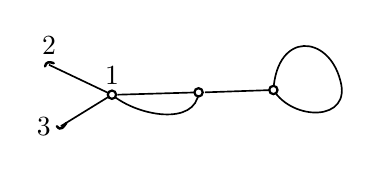
\begin{tikzpicture}[x=1cm,y=1cm,line width=.6pt]
\coordinate (a) at (0,0); \coordinate (b) at (-.8,.38); \coordinate (c) at (-.65,-.4); \coordinate (d) at (1.1,.03); \coordinate (e) at (2.05,.06);
\draw (b)--(a)--(c);
\draw (.07,0)--(d) (1.18,.03)--(e);
\draw (a) to[out=-40,in=-95] (d);
\draw (e) .. controls (2.1,.81) and (2.75,.76) .. (2.9,.18) .. controls (3.05,-.34) and (2.3,-.34) .. (e);
\draw[line width=.9pt,line cap=round] (-.85,.36) .. controls (-.84,.42) and (-.79,.42) .. (-.74,.40);
\draw[line width=.9pt,line cap=round] (-.70,-.40) .. controls (-.65,-.47) and (-.61,-.40) .. (-.58,-.36);
\foreach \p in {a,d,e} {\draw[fill=white,line width=.8pt] (\p) circle (1.5pt);}
\node[above] at (a) {$1$}; \node[above] at (b) {$2$}; \node[left] at (c) {$3$};
\end{tikzpicture}}
\margin{96}
